\section{Task 1}

\subsection{Some equation lol}

We wish to look at reaction-diffusion equations, which have the form
\begin{equation}
    \label{eq:original_eq}
     u_t = \mu u_{xx} + f(u)
\end{equation}
where $\mu$ is a positive constant.
We also assume that the reaction term,
$f(u)$, is a linear function in \( u \).
That is, it can be written as \( f(u) = au \),
for some constant \( a \in \mathbb{R}, a \neq 0 \).
Explicit methods can be used to solve $u_t = f(u)$.

We solve the equation on
the grid \( (x, t) \in [0, 1] \times [0, 1] \)
with boundary conditions given by functions
\( f, g_1 \) and \( g_2 \).
\begin{align*}
  u(0, x) &= f(x) \\
  u(t, 0) &= g_1(t) \\
  u(t, 1) &= g_2(t)
\end{align*}

\subsection{Discretization}

We discretize the domain in both space and time,
such that $x_m = mh$ and $t_n = nk$,
where \( m = 0, 1, \dots, M + 1\) and \( n = 0, 1, \dots, N \)
for some positive constants \( M, N \).

\begin{figure}[!h]
\centering
\label{fig:disc}
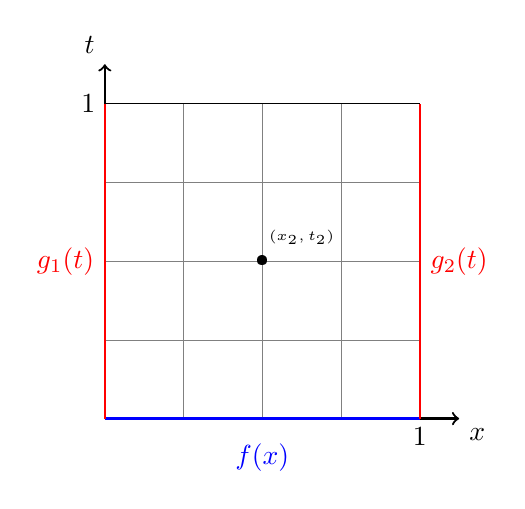
\begin{tikzpicture}
  \draw[help lines] (0,0) grid (4, 4);

  \draw[thick,->] (0,0) -- (4.5,0) node[anchor=north west] {\( x \)};
  \draw[thick,->] (0,0) -- (0,4.5) node[anchor=south east] {\( t \)};

  \draw[very thin] (0,4) node[anchor=east] {\( 1 \)} -- (4,4) ; 
  \draw[very thin] (4,0) node[anchor=north] {\( 1 \)} -- (4,4) ; 

    \node[blue,rectangle] at (2, -0.5) {\( f(x) \)};
    \draw[blue, thick] (0,0) -- (4,0); 

    \node[red,rectangle] at (-0.5,2) {\( g_1(t) \)};
    \node[red,rectangle] at (4.5,2) {\( g_2(t) \)};
    \draw[red, thick] (0,0) -- (0,4); 
    \draw[red, thick] (4,0)  -- (4,4); 

    \node at (2.5,2.3) {\tiny \( (x_2, t_2) \)};
    \node at (2,2) {\textbullet};
\end{tikzpicture}
\caption{The domain \( [0, 1] \times [0, 1] \), with boundary and initial conditions
given by functions \( f, g_1 \) and \( g_2 \).}
\end{figure}

A scheme based on forward and backward Euler,
together with a central difference in space, could be:
$$
  \frac{1}{k}\nabla_tU_{m}^{n+1}=\frac{\mu}{h^2}\delta_x^2U_{m}^{n+1}+f(U_{m}^{n} )
$$
which can be rewritten to 
$$
  U_{m}^{n+1} = U_{m}^{n} + r (U_{m+1}^{n+1}-2U_{m}^{n+1}+U_{m-1}^{n+1}) + kf(U_{m}^{n}), \quad r = \mu\frac{k}{h^2}
$$
Time dependent PDEs with diffusion terms should be solved using implicit methods.
This requires solving a nonlinear system for each step.
The following scheme is based on an implicit method
for the diffusion term and an explicit method for the reaction term.
\begin{align}
  \label{eq:scheme_implicit_eq}
    U_{m}^{*} =& U_{m}^{n} +\frac{r}{2}(\delta_x^2 U_{m}^{*} + \delta_x^2 U_{m}^{n} ) + kf(U_{m}^{n}) \\
  \label{eq:scheme_explicit_eq}
    U_{m}^{n+1} =& U_{m}^{*} + \frac{k}{2}(f(U_{m}^{*}) - f(U_{m}^{n}))
\end{align}

\subsection{Stability analysis}

Define the matrix \( S \) as
\begin{equation}
  \label{eq:Smatrix}
  S = 
  \begin{bmatrix}
    -2 & 1 &  &  & \\
    1& -2 & 1 &  & \\
     & \ddots & \ddots & \ddots & \\
     &  & 1 & -2 & 1\\
     &  &  & 1 & -2\\
  \end{bmatrix}
\end{equation}

and define the vector \( U^n = [U_1^n, U_2^n, \dots, U_M^n]^T \)
by combining the function values at the \( M \) inner points into a vector.
To make the matrix-vector product well defined, let \( S \) be of dimensions
\( M \times M \).

Rewriting equation \ref{eq:scheme_implicit_eq} as a matrix-vector equation
and collecting the \( U^* \)-s on the left hand side yields:
\begin{equation}
  (I - \frac{r}{2}S)U^* = (I + kaI + \frac{r}{2}S) U^n
\end{equation}

\begin{lemma}
  \label{lemma:existance_of_inverse}
  Let \( S \in \text{Mat}_M(\mathbb{R}) \) be defined as in \eqref{eq:Smatrix}.
  Then \( \left(I - \frac{r}{2}S\right)^{-1}\) exists. TODO: for which M, r?
\end{lemma}
\begin{proof}
    jajajjaja
\end{proof}

Now since the inverse of \( I - \frac{r}{2}S \) exists,
we substitute for \( U^* \)
in equation \ref{eq:scheme_explicit_eq}
and arrive at an expression for the matrix \( C \)
satisfying \( U^{n+1} = C U^n \).
\begin{align*}
  U^{n+1} &= U^n + \frac{ka}{2}\left(U^*  - U^n\right) \\
          &= \left(1 + \frac{ka}{2}\right) U^* - \frac{ka}{2}U^n \\
          &= \left(1 + \frac{ka}{2}\right) {\left[I - \frac{r}{2}S\right]}^{-1} \left(I + kaI + \frac{r}{2}S\right) U^n - \frac{ka}{2}U^n \\
          &= {\left[I - \frac{r}{2}S\right]}^{-1} \left(\left(1 + \frac{ka}{2}\right)\left(I + kaI + \frac{r}{2}S\right) - \frac{ka}{2}\left(I-\frac{r}{2}S\right)\right) U^n \\
          &= {\left[I - \frac{r}{2}S\right]}^{-1} \left( \left(1+ka+\frac{1}{2}(ka)^2\right)I + \frac{1}{2}\left(1+ka\right)rS\right) U^n
\end{align*}

So
\begin{equation}
    C = {\left[I - \frac{r}{2}S\right]}^{-1} \left( \left(1+ka+\frac{1}{2}(ka)^2\right)I + \frac{1}{2}\left(1+ka\right)rS\right).
  \end{equation}

\begin{lemma}
  \label{lemma:S_diagonalizable}
  The matrix \( S = \text{tridiag}(1, -2, 1) \in \text{Mat}_{M, M}(\mathbb{R}) \)
  is diagonalizable by a orthogonal matrix \( P \): \( S = P \Lambda P^T \).
  The eigenvalues of \( S \) are
  \( \lambda_m = - \sin^2 \phi_m, \phi_m = \frac{m \pi}{2(M+1)}, m = 1, \dots, M\).
\end{lemma}
\begin{proof}
    duuuh.
\end{proof}

By using lemma \ref{lemma:S_diagonalizable} we arrive at a diagonalization for \( C \):
\begin{align*}
  C &= {\left[I - \frac{r}{2}S\right]}^{-1} \left( \left(1+ka+\frac{1}{2}(ka)^2\right)I + \frac{1}{2}\left(1+ka\right)rS\right) \\
    &= {\left[PP^T - \frac{r}{2}P\Lambda P^T\right]}^{-1} \left( \left(1+ka+\frac{1}{2}(ka)^2\right)PP^T + \frac{1}{2}\left(1+ka\right)r P\Lambda P^T\right) \\
    &= P{\left[I - \frac{r}{2}\Lambda \right]}^{-1} \left( \left(1+ka+\frac{1}{2}(ka)^2\right)I + \frac{1}{2}\left(1+ka\right)r \Lambda \right) P^T \\
    &= P \Delta P^T
\end{align*}
where
\begin{equation}
    \Delta = {\left[I - \frac{r}{2}\Lambda \right]}^{-1} \left( \left(1+ka+\frac{1}{2}(ka)^2\right)I + \frac{1}{2}\left(1+ka\right)r \Lambda \right)
\end{equation}

We observe that \( C \) is symmetric
since \( C = P \Delta P^T = P \Delta^T P^T = \left(P \Delta P^T\right)^T = C^T \).
This is nice since now the condition \( \rho(C) \le 1 + \nu k \) is
both \textit{necessary} and sufficient for stability
when we use \( ||\cdot||_{2,h} \).
In particular, for a symmetric matrix \( C \) we have that \( ||C||_{2,h} = \rho(C) \).

The eigenvalues for \( C \) are found on the diagonal of \( \Delta \):
\begin{equation}
  \Delta_m =
      \frac{\left(1+ka+\frac{1}{2}(ka)^2\right) + \frac{1}{2}\left(1+ka\right)r \lambda_m}
      {1 - \frac{r}{2} \lambda_m}
\end{equation}

A bound on \( \rho(C) = \max_{m} \lvert \Delta_m \rvert \) is found:
\begin{align*}
  \left\lvert \Delta_m \right\rvert &= 
\left\lvert \frac{\left(1+ka+\frac{1}{2}(ka)^2\right) + \frac{1}{2}\left(1+ka\right)r \lambda_m}
{1 - \frac{r}{2} \lambda_m} \right\rvert \\
 &= 
 \left\lvert \left(1+ka\right)\frac{1+\frac{1}{2}r \lambda_m}{1 - \frac{1}{2}r \lambda_m} + \frac{1}{2}(ka)^2 \frac{1}{1 - \frac{1}{2}r \lambda_m} \right\rvert \\
 &\le \left\lvert \left(1+ka\right) \right\rvert \left\lvert \frac{1+\frac{1}{2}r \lambda_m}{1 - \frac{1}{2}r \lambda_m} \right\rvert + \frac{1}{2}(ka)^2 \left\lvert\frac{1}{1 - \frac{1}{2}r \lambda_m} \right\rvert \\
 \intertext{
   Note that \( -1 < \lambda_m < 0  \) for all \( m = 1, \dots, M \).
   In addition, the step size \( k \) is bounded by some constant
   \( T \) (having a step size larger than the length of the time domain
   does not make sence).
  We can simplify further:
}
 \left\lvert \Delta_m \right\rvert
 &\le 1 + (\lvert a \rvert + \frac{1}{2}k a^2 )k \\
 &\le 1 + (\lvert a \rvert + \frac{1}{2}T a^2)k \\
 &= 1 + \nu k
\end{align*}

And now we have arrived at the expression needed for stability
without imposing any conditions on the scheme.
We summarize our discussion in a theorem.

\begin{theorem}
  The scheme given in equations \ref{eq:scheme_implicit_eq} and \ref{eq:scheme_explicit_eq} is unconditionally stable.
\end{theorem}

\subsection{Consistency}

\begin{lemma}
    \label{central_difference}
    $$\delta_x^2u_{m}^{n} = h^2\partial_x^2 u_{m}^{n} + \mathcal{O}(h^4)$$
\end{lemma}
\begin{proof}
    left as an exercise to the reader.
\end{proof}

\begin{theorem}
    \label{consistent}
    Given that $u$ is sufficiently smooth,  $f$ is of the form $f(u)=au, a\in \mathbb{R}$ and $k \neq \frac{-2}{a}$, the local truncation error of the method is $\mathcal{O}(k^2 + h^2).$
\end{theorem}

\begin{proof}
    We rewrite (\ref{eq:scheme_explicit_eq}) to be an explicit equation for $U_m^*$
    $$ U_{m}^{*}= \frac{U_{m}^{n+1}+\frac{ka}{2}U_{m}^{n}}{1+\frac{ka}{2}}.$$
    This is then substituted into \ref{eq:scheme_implicit_eq} to remove $U_{m}^{*}$ from the equation
    $$\frac{U_{m}^{n+1}+\frac{ka}{2}U_{m}^{n}}{1+\frac{ka}{2}} = (1+ka)U_{m}^{n}+\frac{r}{2}\left( \frac{\delta_x^2(U_{m}^{n+1}+\frac{ka}{2}U_{m}^{n})}{1+\frac{ka}{2}}  + \delta_x^2 U_{m}^{n}\right).$$
    We then multiply by $(1+\frac{ka}{2})$ and rearrange the terms to
    $$ U_{m}^{n+1}=(1+ ka + \frac{k^2a^2}{2})U_{m}^{n} + \frac{r}{2}\left((1+ka)\delta_x^2U_{m}^{n} +\delta_x^2U_{m}^{n+1}\right).$$
    Then the approximations are replaced by $u$ and the local truncation error is therefore introduced
    $$ k\tau_m^n + u_{m}^{n+1} = (1+ ka + \frac{k^2a^2}{2})u_{m}^{n} + \frac{r}{2}\left((1+ka)\delta_x^2u_{m}^{n} +\delta_x^2u_{m}^{n+1}\right).$$
    We then use lemma (\ref{central_difference}) for the central differences and Taylor expand around $u_{m}^{n}$
    \begin{align*}
        k \tau_m^n =& \left( 1 + ka +\frac{k^2a^2}{2}\right)u_{m}^{n} - u_{m}^{n+1}+\frac{\mu k}{2h^2} \left(h^2\partial_x^2 u_{m}^{n+1} + \left( 1+ka \right) h^2 \partial_x^2u_{m}^{n} + \mathcal{O}(h^4)\right) \\
        k \tau_m^n =& \left( 1 + ka + \frac{k^2a^2}{2}\right)u_{m}^{n} - u_{m}^{n} - k \partial_tu_{m}^{n} - \frac{k^2}{2} \partial_t^2 u_{m}^{n} + \mathcal{O}(k^3)  \\
        +& \frac{\mu k}{2}\left( \partial_x^2 \left( u_{m}^{n} + k \partial_t u_{m}^{n} + \mathcal{O}(k^2)\right) + \left( 1 + ka\right) \partial_x^2  u_{m}^{n} \right) + \mathcal{O}(kh^2).
    \end{align*}
    This expression is then divided by $k$ and rearranged to 
    $$\tau_m^n = a u_{m}^{n} - \partial_tu_{m}^{n} + 2 \frac{\mu}{2}\left( \partial_x^2 u_{m}^{n}\right) +  \frac{ka^2}{2}u_{m}^{n}  - \frac{k}{2} \partial_t^2 u_{m}^{n} + \frac{\mu }{2}\left( k \partial_x^2 \partial_t u_{m}^{n}  + ka \partial_x^2  u_{m}^{n} \right) + \mathcal{O}(h^2 + k^2).$$
    The first three terms are simply (\ref{eq:original_eq}) with all terms moved to the right hand side. Some terms can also be rewritten using (\ref{eq:original_eq}), $\mu \partial_x^2u_{m}^{n} = \partial_t u_{m}^{n} - au_{m}^{n}$, yielding
    \begin{align*}
        \tau_m^n = \frac{ka^2}{2}u_{m}^{n}  - \frac{k}{2} \partial_t^2 u_{m}^{n} +& \frac{k}{2} \partial_t \left(\partial_t u_{m}^{n}   - au_{m}^{n} \right) + \frac{ka}{2} \left( \partial_t  u_{m}^{n} - a u_{m}^{n}\right)+ \mathcal{O}(h^2 + k^2) \\
        \tau_m^n = \frac{ka^2}{2}u_{m}^{n} - \frac{ka^2}{2}u_{m}^{n}  -& \frac{k}{2} \partial_t^2 u_{m}^{n} + \frac{k}{2} \partial_t^2 u_{m}^{n} - \frac{ak}{2} \partial_t u_{m}^{n} + \frac{ka}{2} \partial_t  u_{m}^{n}+ \mathcal{O}(h^2 + k^2) \\
        \tau_m^n =& \mathcal{O}(h^2 + k^2) \\
    \end{align*}
\end{proof}

\begin{theorem}
    Given that $u$ is sufficiently smooth,  $f$ is of the form $f(u)=au, a\in \mathbb{R}$ and $k \neq \frac{-2}{a}$, the method is convergent.
\end{theorem}

\begin{proof}
    The method is stable, (\ref{stability}), and consistent, (\ref{consistent}), and therefore convergent by Lax' equivalence theorem.
\end{proof}
\subsection{Numerical experiments}

We use the following test equation:
\begin{align}
  u_t &= \frac{1}{5}u_xx + 5 u \\
  u(0, x) &= \sin (2\pi x) \\
  u(t, 0) &= 0 \\
  u(t, 1) &= 0
\end{align}

The solution is
\begin{equation}
  \label{eq:anal_sol}
  u(t, x) = \text{e}^{-(4\pi^2 \mu - a)t}\sin(2\pi x)
\end{equation}

\begin{figure}[h]
    \centering
    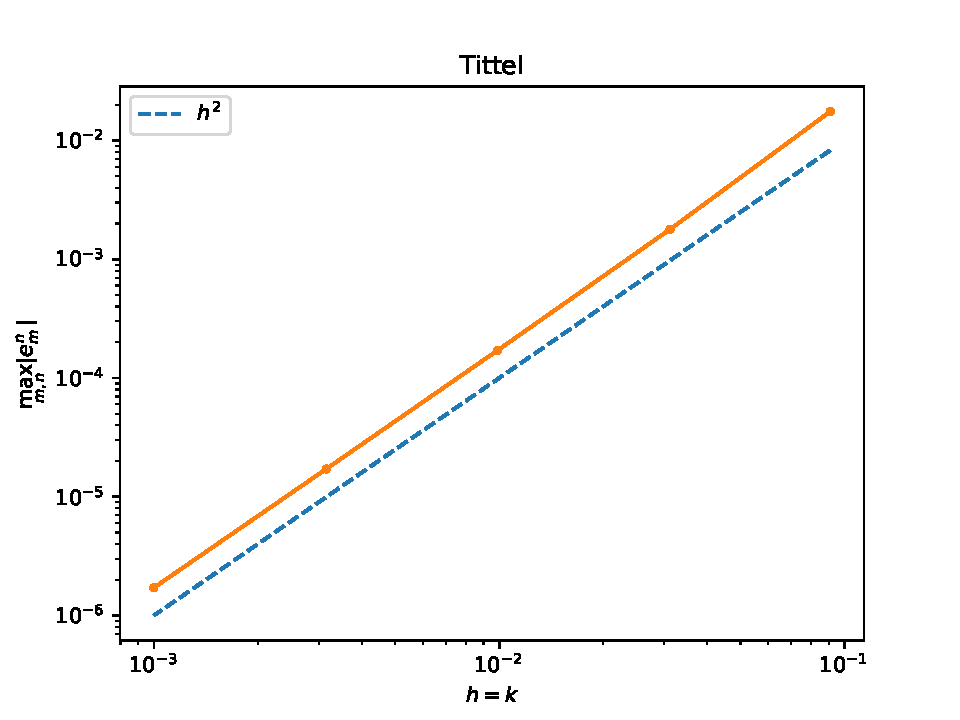
\includegraphics[width=0.75\textwidth]{Images/plots/temp_task1.pdf}
    \caption{TEMP: convergence plot}
    \label{fig:mesh1}
\end{figure}
